\documentclass{scrreprt}
\usepackage[english]{babel}
\usepackage[T1]{fontenc}
\usepackage{lmodern}
\usepackage{blindtext}
\usepackage[utf8]{inputenc}
\usepackage{siunitx} %For unit handling%
\renewcommand{\familydefault}{\sfdefault}
\newcommand{\unit}[1]{\ensuremath{\, \mathrm{#1}}}
\usepackage{amssymb, amsmath, cancel, ulem, graphicx, float, tabularx, multirow, bm}
\usepackage{amsmath}
\usepackage{caption}
\usepackage{subcaption}
\usepackage{mathtools}
\usepackage{tikz}
\newcommand*\circled[1]{\tikz[baseline=(char.base)]{
            \node[shape=circle,draw,inner sep=1pt] (char) {#1};}}
\renewcommand{\phi}{\varphi}


\setcounter{secnumdepth}{5}
\setcounter{tocdepth}{5}

\author{Urs Gerber\\09-921-156 \and Gian-Luca Mateo\\11-113-545}
\date{18th of April 2013}

\title{Coupled pendulums}
\subtitle{Practical course report}

\begin{document}

\maketitle

\tableofcontents
\newpage

\chapter{Experiment: Coupled pendulums}

\section{Introduction}

\subsection{Goal of the experiment}
The goal of this experiment is to measure and analyse the characteristics of a coupled pendulum. For that we measure the cycle duration of the coupled pendulum in three different oscillation modes: in-phase, opposite in-phase and paraphase.

\subsection{Theory}

\subsubsection{Mathematical pendulum}
The equation of motion for the mathematical pendulum with thread length $l$ is given by
\begin{equation}
\ddot{\phi} + \frac{g}{l} \cdot \sin{\phi} = 0 \xRightarrow{\sin{\phi}\approx\phi} \ddot{\phi} + \frac{g}{l} \cdot \phi = 0
\end{equation}
with solution 
\begin{equation}
\phi (t) = \hat{\phi} \cdot \sin{\left( \sqrt{\frac{g}{l}} \cdot t + \phi_0 \right)} 
\end{equation}
The oscillation period $T_0$ of the mathematical pendulum is
\begin{equation}
T_0 = 2 \pi \sqrt{\frac{l}{g	}}
\end{equation}

\subsubsection{Coupled physical pendulum}

The equation of motion for one physical pendulum is given by

\begin{equation}
J\cdot \ddot{\phi} = M
\end{equation}
where $J$ is the moment of inertia with respect to the axis of rotation $O$ and $M$ the repulsive angular moment.

The moment equations for pendulum 1 and pendulum 2 are:
\begin{align}
M_1 &= \overbrace{-D_g\cdot \phi_1}^{\text{directional moment}} + \overbrace{D_f \cdot (\phi_1 - \phi_2)}^{\text{coupling moment}}  \\
M_2 &= -D_g\cdot \phi_2 - D_f \cdot (\phi_1 - \phi_2)
\end{align}

After inserting the moment equations into the equation of motion and solving the differential equations, we get the two solutions

\begin{align}
\phi_1(t) &= A \cdot \cos{(\omega t + \delta)} - B \cdot \cos{(\Omega t + \Delta)}\\
\phi_2(t) &= A \cdot \cos{(\omega t + \delta)} + B \cdot \cos{(\Omega t + \Delta)}
\end{align}
with natural frequencies $\omega$ and $\Omega$
\begin{align}
\omega &= \sqrt{\frac{D_g}{J}}\\
\Omega &= \sqrt{\frac{D_g+2 D_f}{J}}
\end{align}
One can see that the overall motion of each pendulum is composed of a superposition of two harmonic oscillations with different frequencies (beat).

\paragraph{Moment of inertia $J$}
The moment of inertia $J$ of one pendulum can be found by summing up the share of the shaft $J_s$, weight $J_w$ and nut $J_n$:

\begin{equation}
J = J_s + J_w + J_n
\end{equation}

The formulae for $J_s$, $J_w$ and $J_n$ can be found in the script on page 103 ff:

\begin{align}
J_s &= \frac{m_s}{12} \left( 3 r^2 + 4 l^2 \right)\\
J_w &= \frac{m_g}{12} \left[ 3(R^2 + r^2) + h^2 +12d^2 \right]\\
J_n &= \frac{m_n}{12} \left[ 3 ( R_R^2+r_R^2) + h'^2+12d'^2 \right]
\end{align}

\paragraph{Initial values}
We distinguish the following three cases for pendulum 1 and pendulum 2. At $t=0$ the initial deflections of the pendulums may be
\begin{itemize}
\item in-phase: $\phi_1 = \Phi, \quad \phi_2 = \Phi$
\item opposite in-phase: $\phi_1 = -\Phi, \quad \phi_2 = +\Phi$
\item paraphase: $\phi_1 = 0, \quad \phi_2 = \Phi$
\end{itemize}

\subparagraph*{In-phase}
The solutions in the in-phase case are
\begin{align}
\phi_1(t) &= \Phi \cos{\omega t}\\
\phi_2(t) &= \Phi \cos{\omega t}
\end{align}
with oscillation period $\tau_{\omega}$
\begin{equation}
\tau_{\omega} = \frac{2 \pi}{\omega} = 2 \pi \sqrt{\frac{J}{D_g}}
\end{equation}

\subparagraph*{Opposite in-phase}
The solutions in case of opposite in-phase mode are
\begin{align}
\phi_1(t) &= -\Phi \cos{\omega t}\\
\phi_2(t) &= \Phi \cos{\omega t}
\end{align}
with oscillation frequency $\tau_{\Omega}$
\begin{equation}
\tau_{\Omega} = \frac{2 \pi}{\Omega} = 2 \pi \sqrt{\frac{J}{D_g+2 D_f}}
\end{equation}

\subparagraph*{Paraphase}
The solutions for the paraphase case are
\begin{align}
\phi_1(t) &= \frac{\Phi}{2}\left(\cos{\omega t} - \cos{\Omega t}\right)\\
\phi_2(t) &= \frac{\Phi}{2}\left(\cos{\omega t} + \cos{\Omega t}\right)
\end{align}
with oscillaiton frequency $\tau$ and beat frequency $T_s$
\begin{align}
\tau &= \frac{4 \pi}{\Omega + \omega}\\
T_s &= \frac{2 \pi}{\Omega -\omega}
\end{align}
Both $\tau$ and $T_s$ can be expressed in dependance of $\tau_{\omega}$ and $\tau_{\Omega}$ via
\begin{align}
\frac{1}{\tau} &= \frac{1}{2}\left( \frac{1}{\tau_{\omega}} + \frac{1}{\tau_{\Omega}} \right)\label{tau}\\
\frac{1}{T_s} &= \frac{1}{\tau_{\Omega}} - \frac{1}{\tau_{\omega}}\label{ts}
\end{align}

\paragraph*{Degree of coupling}
The degree of coupling $k$ between the two pendulums can be found either statically

\begin{equation} \label{eq:coupconst_stat}
k = \frac{\Phi_1}{\Phi_2}
\end{equation}

or dynamically

\begin{equation} \label{eq:coupconst_dyn}
k = \frac{\tau_{\omega}^2 - \tau_{\Omega}^2}{\tau_{\omega}^2 + \tau_{\Omega}^2}
\end{equation}

\paragraph*{Coupling moment}
The coupling moment $D_f$ can also be determined statically

\begin{equation} \label{eq:coupling_stat}
D_f = g l \left( m+ \frac{m'}{2} \right) \frac{\Phi_1}{\Phi_2 -\Phi_1}
\end{equation}

or dynamically

\begin{equation} \label{eq:coupling_dyn}
D_f = 2 \pi^2 J \left( \frac{1}{\tau_{\Omega}^2} - \frac{1}{\tau_{\omega}^2}  \right) 
\end{equation}


\subsection{Uncertainty analysis}
Our uncertainty analysis is based on statistical methods such as standard deviation and standard error of the mean in case of measured quantities. For derived quantities the following section lists all formulae used to obtain the errors in our calculations.

\subsubsection{Degree of coupling}
\paragraph*{Static}
\begin{equation}
s_k^2 = \frac{\Phi_2^2 s_{\Phi_1}^2 + \Phi_1^2 s_{\Phi_2}^2}{\Phi_2^4}
\end{equation}

\paragraph*{Dynamic}
\begin{equation}
s_k^2 = \frac{16 \left( s_{\tau_{\Omega}}^2 \tau_{\omega}^4 \tau_{\Omega}^2 + s_{\tau_{\omega}}^2 \tau_{\omega}^2 \tau_{\Omega}^4 \right)}{\left( \tau_{\omega}^2+ \tau_{\Omega}^2 \right)^4}
\end{equation}

\subsubsection{Oscillation period $\tau$}
\begin{equation}
s_{\tau}^2 = \frac{4 \left( s_{\tau_{\Omega}}^2 \tau_{\omega}^4 + s_{\tau_{\omega}}^2 \tau_{\Omega}^4 \right)}{\left( \tau_{\omega}+ \tau_{\Omega} \right)^4}
\end{equation}

\subsubsection{Beat period $T_s$}
\begin{equation}
s_{T_s}^2 = \frac{s_{\tau_{\Omega}}^2 \tau_{\omega}^4 + s_{\tau_{\omega}}^2 \tau_{\Omega}^4 }{\left( \tau_{\omega} - \tau_{\Omega} \right)^4}
\end{equation}

\subsubsection{Coupling moment $D_f$}

\paragraph*{Static}
\begin{equation}
s_{D_f}^2 = \frac{g^2 l^2 \left(2 m + m'\right)^2 \left( \Phi_2^2 s_{\Phi_1}^2 + \Phi_1^2 s_{\Phi_2}^2 \right)}{4 \left(\Phi_1 -\Phi_2\right)^4} 
\end{equation}

\paragraph*{Dynamic}
\begin{equation}
s_{D_f}^2 = \frac{16 J^2 \pi^6 \left( s_{\tau_{\Omega}}^2 \tau_{\omega}^6 + s_{\tau_{\omega}}^2 \tau_{\Omega}^6 \right)}{\tau_{\omega}^6 \tau_{\Omega}^6}
\end{equation}

\section{Experiment setup and execution}

\subsection{Used materials}
The materials used in this experiment are the following:
\begin{itemize}
\item An assembly (labelled No.$3$) with two ball bearing mounted shafts ($m_s = 21.37\unit{g}$ each), which have threaded bottoms
\item Two weights ($m_w = 214.15 \unit{g}$ each) with threaded holes which can be screwed onto the bottom of the shafts and secured with two nuts ($m_n = 2\unit{g}$ each)
\item two brackets, mountable to the shafts
\item a spring, attachable to the brackets 
\item a ruler, metric scale, $38 \unit{cm}$ long
\item a mechanical stopwatch, $0.2 \unit{s}$ steps
\end{itemize}

\subsection{Assembly}
For our measurements, the materials are assembled as shown in image \ref{fig:assembly}.

\begin{figure}[H]
	\centering
  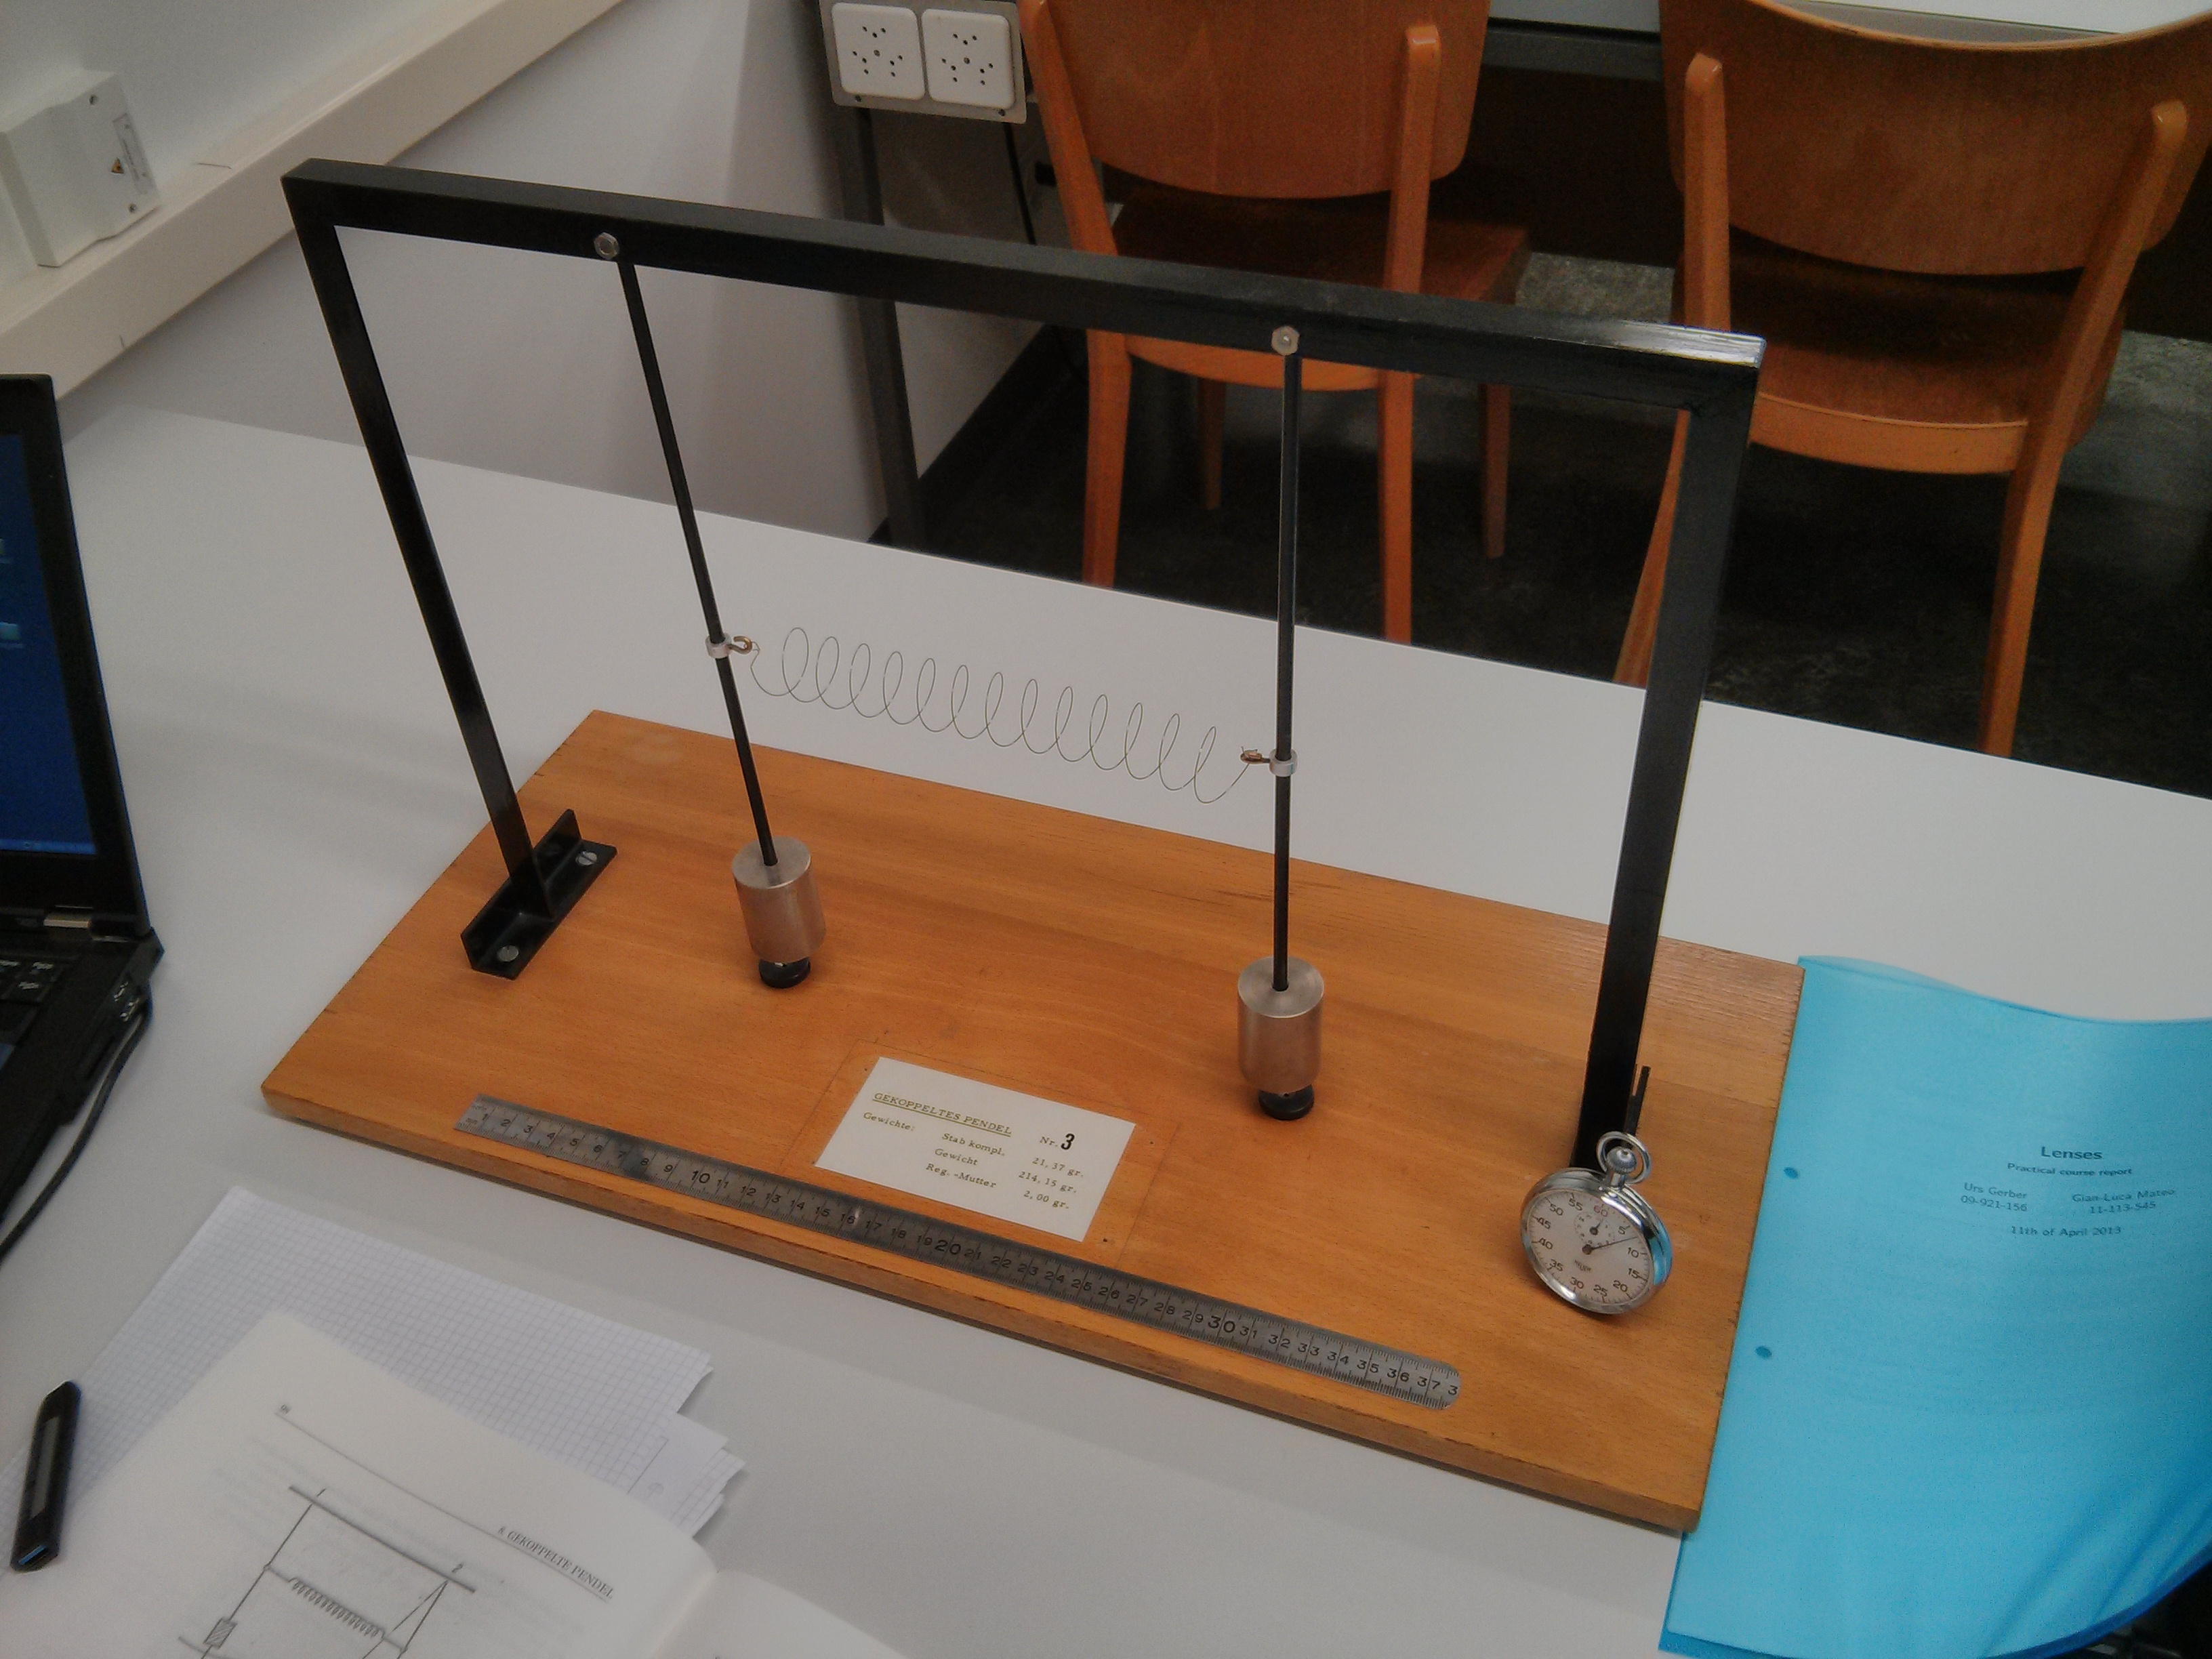
\includegraphics[width=0.9\textwidth]{img/assembly.jpg}
	\caption{Experiment Assembly}
	\label{fig:assembly}
\end{figure}
For the first series of measurements, one pendulum is detached from the spring, deflected and its oscillation period measured. for the second series, the weight at the bottom of the second pendulum is moved up or down in order to obtain the same period as the first one. Next, the spring is attached to both pendulums at the same height. Once this is done, the following values are measured:
\begin{itemize}
\item $\tau_{\omega}$: in-phase oscillation period, $\phi_1 = \phi_2$
\item $\tau_{\Omega}$: opposite in-phase oscillation period, $\phi_1 = -\phi_2$
\item $\tau$ : paraphase oscillation period, $\phi_1 = 0, \phi_2 = \Phi$
\item $T_s$ : beat period (the time spent between two stops of a pendulum)
\end{itemize}
\section{Measurements}

\begin{figure}[H]
	\centering
  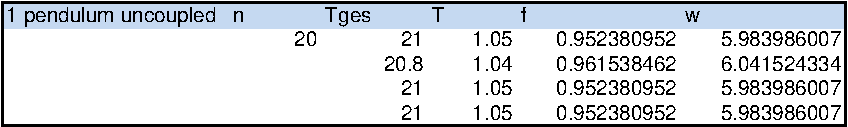
\includegraphics[width=0.9\textwidth]{diag/uncoupled.pdf}
	\caption{Measurements with the spring left unattached}
	\label{fig:uncoupled}
\end{figure}

\begin{figure}[H]
	\centering
  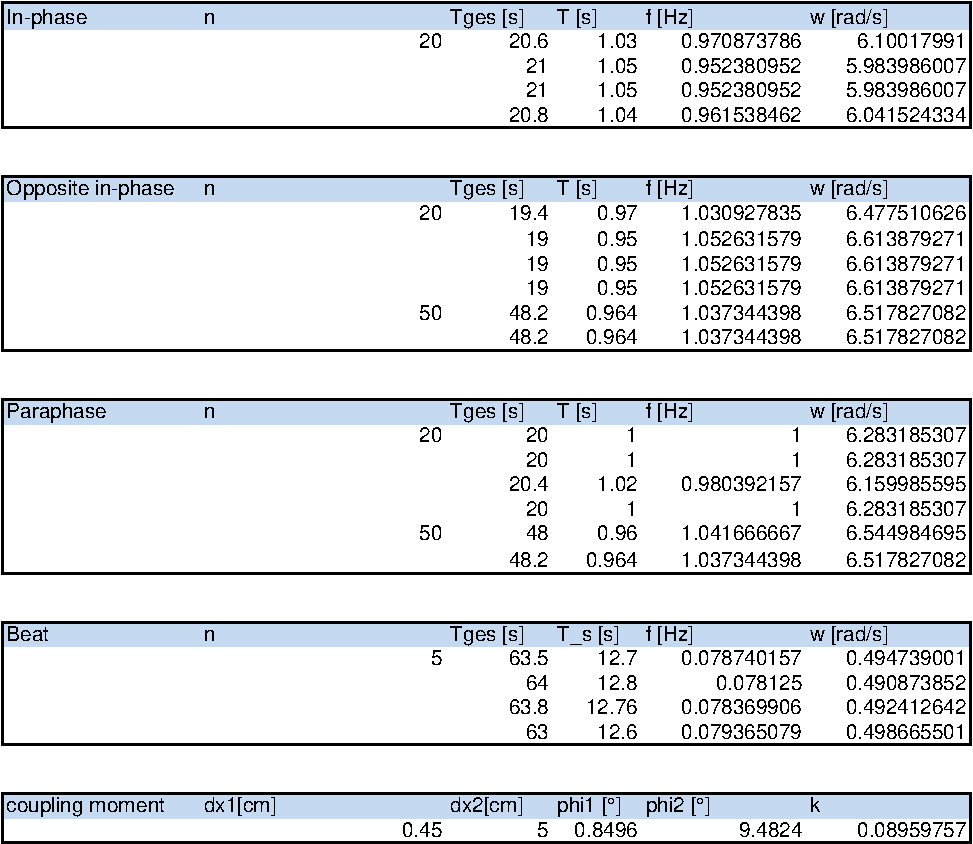
\includegraphics[width=0.9\textwidth]{diag/readings20cm.pdf}
	\caption{Measurements with the spring attached at $20\unit{cm}$ from the top}
	\label{fig:20cm}
\end{figure}

\begin{figure}[H]
	\centering
  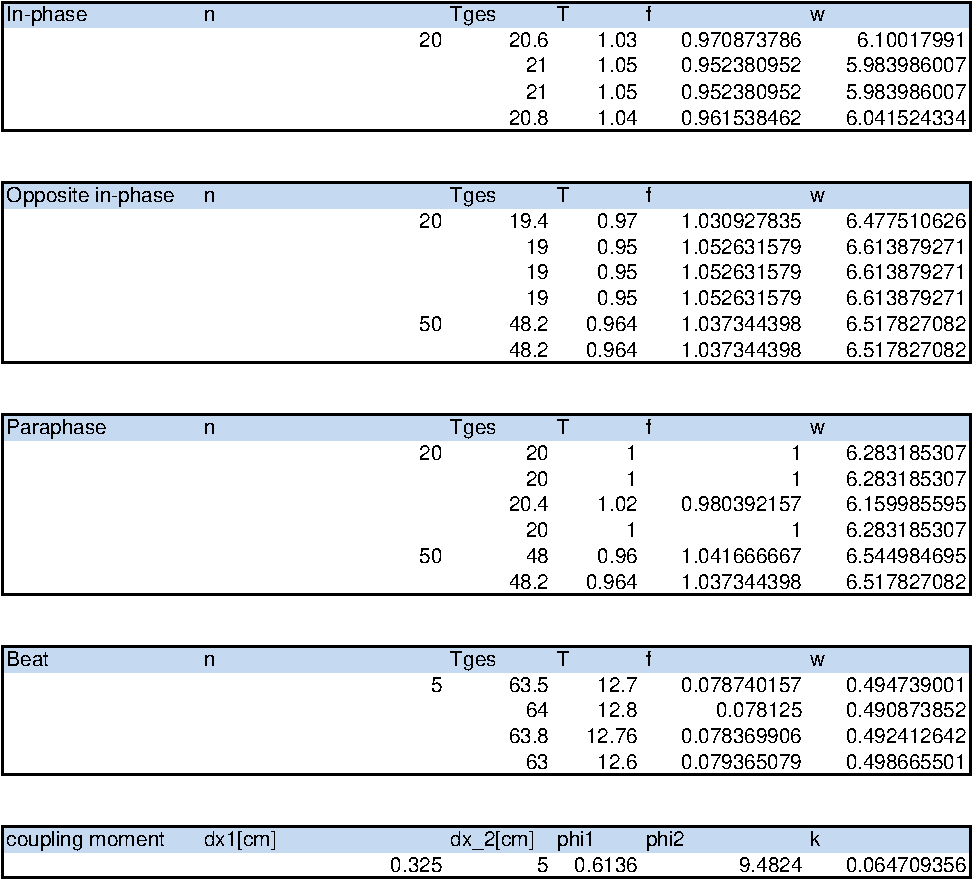
\includegraphics[width=0.9\textwidth]{diag/readings15cm.pdf}
	\caption{Measurements with the spring attached at $15\unit{cm}$ from the top}
	\label{fig:15cm}
\end{figure}
\begin{table}[H]
	\centering
	\begin{tabular}{lcr}		
		$d$&:&$27.2\pm 0.05\unit{cm}$\\
		$l$&:&$30.35\pm 0.05\unit{cm}$\\
		\end{tabular}
	\caption{measured lengths of the pendulum}
\end{table}

\section{Analysis and Discussion}

\begin{table}[H]
\centering
	\begin{tabular}{lcrr}
	&&$h_s = 15\unit{cm}$&$h_s = 20\unit{cm}$\\
	\hline	
	$\tau_\omega$&:&$1.04\pm 0 \unit{s}$&$1.0425\pm 0.00478\unit{s}$\\	
	$\tau_\Omega$&:&$0.994\pm 0.002 \unit{s}$&$0.958\pm 0.00368\unit{s}$\\
	$\tau$&:&$0.996\pm 0.002 \unit{s}$&$0.991\pm 0.00961\unit{s}$\\
	$T_s$&:&$13.24\pm 0.0163 \unit{s}$&$22.0667\pm 0.0272\unit{s}$\\
	\end{tabular}
	\caption{The measured oscillation periods for two different heights of the spring}
\end{table}
\begin{table}[H]
	\centering
	\begin{tabular}{lcr}
		$T_0$&:&$1.0475	\pm 0.0025$
	\end{tabular}
	\caption{Measured oscillation period for the uncoupled pendulum}
\end{table}

\subsection{Free oscillation}
First, we compare the theoretical oscillating period of a mathematical pendulum 
\begin{equation}
	T_m=2\pi\sqrt{\frac{d}{g}}
\end{equation}
to the value $T_0$ we obtained in our measurements for the uncoupled pendulum.
\begin{table}[H]
	\centering
	\begin{tabular}{llr}
		$T_m$&$T_0$&rel. difference\\ \hline
		$1.0462 \unit{s}$&$1.0475 \pm 0.0025$ & $+0.12\%$
	\end{tabular}
	\caption{Measured oscillation period vs mathematical pendulum}
\end{table}
This results show that the approximation for a mathematical pendulum yields values very close to our measurements. This is not a big surprise, as nearly $90\%$ of the mass of the pendulum are contained in the weight at the bottom ($214.15\unit{g}$ out of $237.52\unit{g}$), causing the shaft to have a nearly irrelevant impact on the oscillation period.
\subsection{Coupled oscillation}
Next, we proceed to comparing the measured values of $\tau$ and $T_s$ to the theoretical results obtained using the measured values $\tau_\omega$ and $\tau_\Omega$ and formulae \ref{tau} and \ref{ts}.
\begin{table}[H]
	\centering
	\begin{tabular}{lcrrr}
	&&Calculated&Measurements&relative error\\ \hline
	$\tau$&:& $1.0165 \pm	0.001046 \unit{s}$&$0.998 \pm 0.002 \unit{s}$&$-1.82\% $\\
	$T_s$ &:& $22.473  \pm 1.0223\unit{s}$ &$22.0667 \pm 0.0272\unit{s}$ & $-1.81\%$\\
	\end{tabular}
	\caption{comparison chart for spring attached at 15cm}
\end{table}

\begin{table}[H]
	\centering
	\begin{tabular}{lcrrr}
	&&Calculated&Measurements&relative error\\  \hline
	$\tau$&:& $0.998 \pm 0.00297 \unit{s}$&$0.991 \pm	0.00961\unit{s}$&$-0.71\% $\\
	$T_s$ &:& $11.819 \pm 0.8329\unit{s}$ &$12.715 \pm	0.0435\unit{s}$ & $+7.58\%$\\
	\end{tabular}
	\caption{comparison chart for spring attached at 20cm}
\end{table}

The calculated values are in agreement with our measurements, even though that does not mean a lot for the beat period $T_s$, as the relative errors of the calculated values are nearly $5\%$ and $10\%$, respectively. The stopwatch at our disposal only measured time in $0.2\unit{s}$ steps, which we think is a reason for the big errors. Another reason was that measuring the beat frequency was hard, because after some cycles the pendulums failed to stop completely, which meant we could not know when exactly to stop the watch.

\subsection{Moment of inertia $J$}
We calculated the following moments of inertia for the different components of our pendulums:
\begin{table}[H]
	\centering
	\begin{tabular}{lcr}
	$J_w$&=&$0.0159\unit{kg \cdot m^2}$\\
	$J_s$&=&$0.000656\unit{kg \cdot m^2}$\\
	$J_n$&=&$0.000173\unit{kg \cdot m^2}$
	\end{tabular}
	\caption{calculated moments of inertia}
\end{table}

\subsection{Coupling moment $D_f$}
We now continue to compare the coupling moment $D_f$ measured statically and dynamically. In the static case, the coupling moment can be found with formula \ref{eq:coupling_stat} and the dynamic values were obtained using formula \ref{eq:coupling_dyn}:

\begin{table}[H]
\center
\begin{tabular}{cccc}
 & $D_f$ static & $D_f$ dynamic & rel. difference\\
\hline
$h_s = 20 \unit{cm}$ & $0.0659 \pm 0.0171$ & $0.0559 \pm 0.0123$ & $-15.17\%$\\
$h_s = 15 \unit{cm}$ & $0.0463 \pm 0.0162$ & $0.0289 \pm 0.00422$ & $-37.6\%$\\
 
\end{tabular}
\end{table} 

As one can easily see the values in the dynamic case are significantly lower than their statically obtained counterparts. Although the static values have a higher margin of error we think that the dynamic values are less trustworthy. First, the measurement of the moment of inertia $J$ depicts a significant error on the dynamic values because of the linear relationship of $D_f$ and $J$. If $J$ was not measured accurately, $D_f$ is inherently imprecise as well. Furthermore, the spring coupling the two pendulums together is not ideal and was sometimes fully relaxed or even exerted a repellant force on the pendulums when the pendulums were closest to each other, resulting in a significantly lowered coupling moment than expected.

\subsection{Coupling constant $k$}
The coupling constant $k$ is again measured and calculated statically and dynamically via formlae \ref{eq:coupconst_stat} and \ref{eq:coupconst_dyn} respectively:

\begin{table}[H]
\center
\begin{tabular}{cccc}
 & $k$ static & $k$ dynamic & rel. difference\\
\hline
$h_s = 20 \unit{cm}$ & $0.0896 \pm 0.0212$ & $0.0843 \pm 0.00595$ & $-5.91\%$\\
$h_s = 15 \unit{cm}$ & $0.0647 \pm 0.0211$ & $0.0452 \pm 0.00201$ & $-30.14\%$\\
 
\end{tabular}
\end{table} 

The discrepancies between the static and dynamic values are explained by the same reasonings as in the case of the coupling moment $D_f$.


\section{Conclusion}
Generally speaking, our results strongly agree with theory. The only divergences we noted were very probably due the spring, which we think does not act as theory expects.

\begin{thebibliography}{9}

\bibitem{physcript13}
  Peter Wurz,
  \emph{Anleitung zum Physikpraktikum}
  FS2013

\end{thebibliography}

\end{document}
